\documentclass[tikz,border=10pt]{standalone}
\usetikzlibrary{arrows.meta,backgrounds,calc}
\definecolor{route}{RGB}{31,78,121}
\definecolor{gate}{RGB}{196,64,44}
\definecolor{corefill}{RGB}{233,239,247}
\definecolor{outside}{RGB}{120,120,120}
\begin{document}
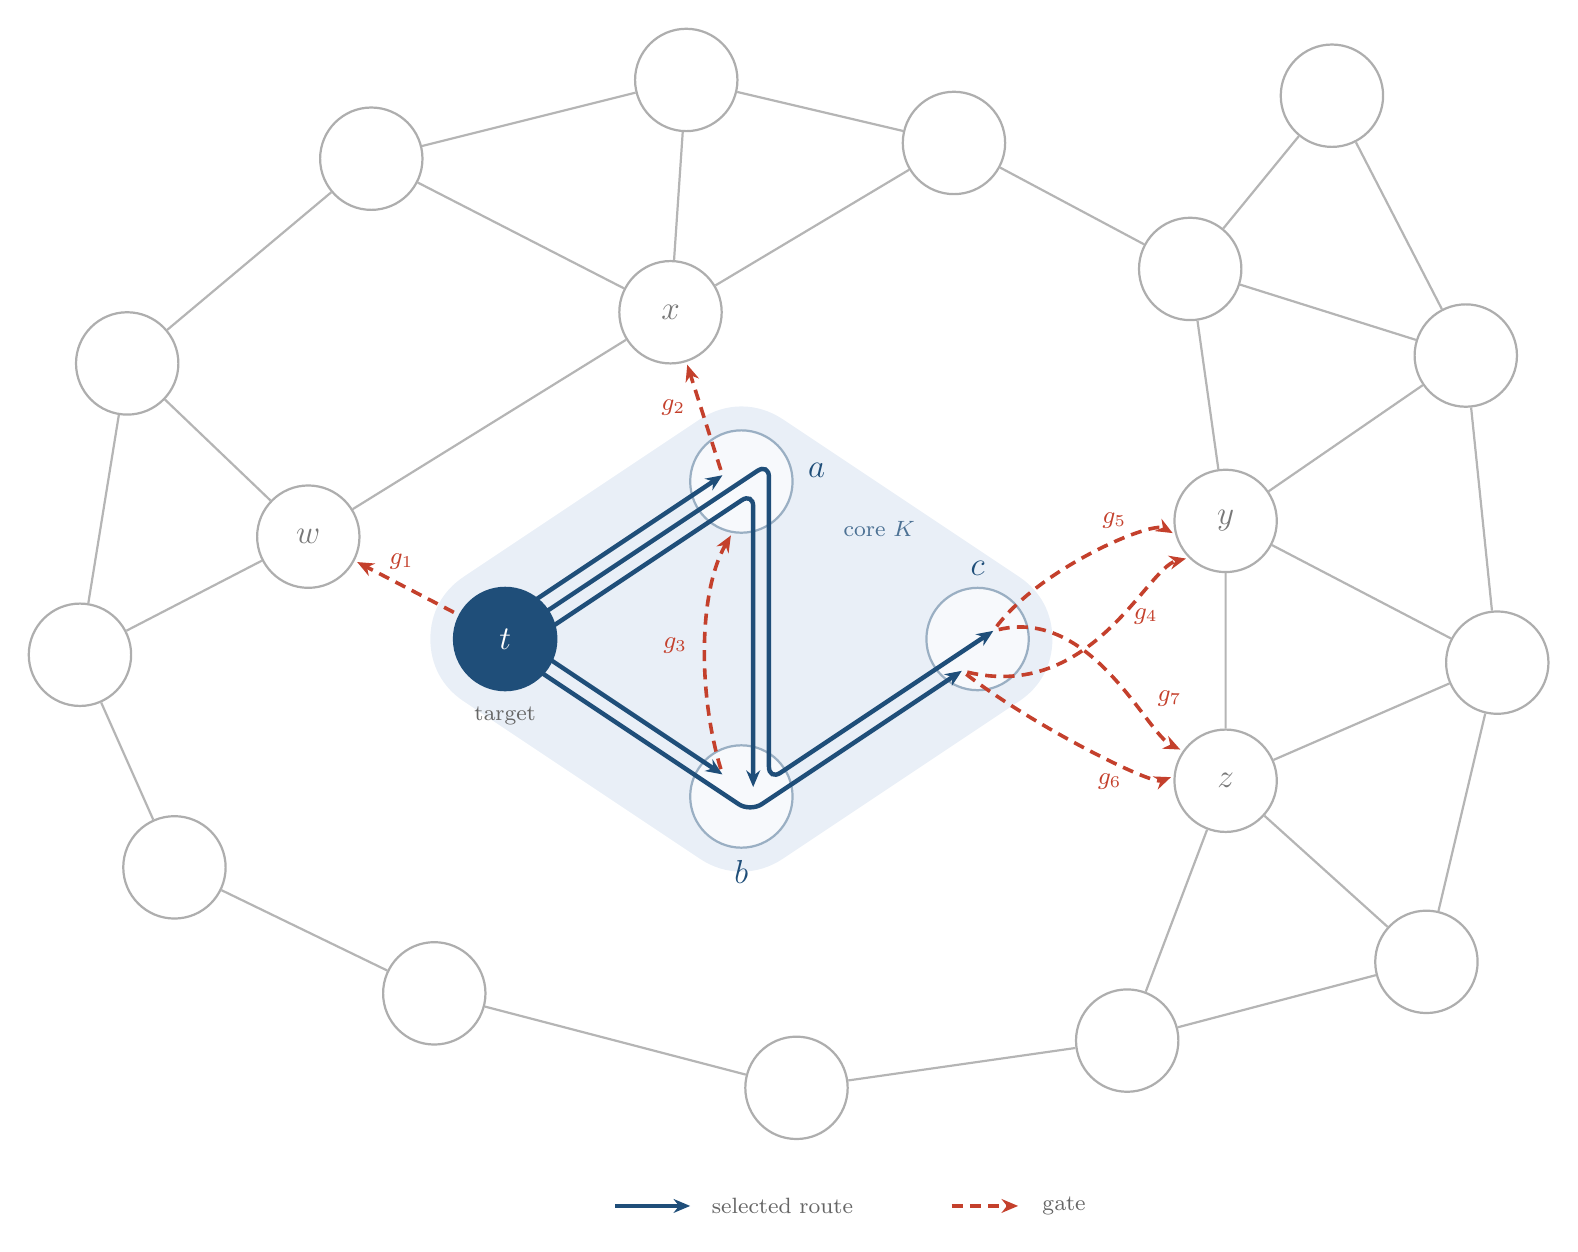
\begin{tikzpicture}[
  >={Stealth[length=6pt,width=5pt]},
  vertex/.style={circle,minimum size=1.3cm,inner sep=0pt,font=\large},
  core/.style={vertex,draw=route!45,fill=white!65!corefill,line width=0.8pt},
  target/.style={vertex,draw=route,fill=route,text=white,line width=0.8pt},
  outer/.style={vertex,draw=outside!60,fill=white,text=outside,line width=0.8pt},
  strand/.style={route,line width=1.6pt,rounded corners=5pt,->},
  gateedge/.style={gate,line width=1.3pt,dash pattern=on 4pt off 2.6pt,->,
                   shorten <=2pt,shorten >=1pt},
  vlabel/.style={font=\large,text=route,inner sep=2pt},
  glabel/.style={font=\small,text=gate,inner sep=2pt},
  note/.style={font=\footnotesize,text=black!60}
]
% Vertices (all the same size) sit behind the strands.
\begin{scope}[on background layer]
% Core region: the convex hull of the core vertices, padded by PAD.
\fill[corefill] (0.000,0.000) -- (3.000,2.000) -- (6.000,0.000) -- (3.000,-2.000) -- cycle;
\draw[corefill,line width=1.9cm,line join=round]
  (0.000,0.000) -- (3.000,2.000) -- (6.000,0.000) -- (3.000,-2.000) -- cycle;
\node[target] (t) at (0.000,0.000) {$t$};
\node[core]   (a) at (3.000,2.000) {};
\node[core]   (b) at (3.000,-2.000) {};
\node[core]   (c) at (6.000,0.000) {};
\node[outer]  (w) at (-2.500,1.300) {$w$};
\node[outer]  (x) at (2.100,4.150) {$x$};
\node[outer]  (y) at (9.150,1.500) {$y$};
\node[outer]  (z) at (9.150,-1.800) {$z$};
\draw[outside!55,line width=0.8pt] (w) -- (x)  (y) -- (z);
\node[outer] (p1) at (-5.400,-0.200) {};
\node[outer] (p2) at (-4.800,3.500) {};
\node[outer] (p3) at (-1.700,6.100) {};
\node[outer] (p4) at (2.300,7.100) {};
\node[outer] (p5) at (5.700,6.300) {};
\node[outer] (p6) at (8.700,4.700) {};
\node[outer] (p7) at (12.200,3.600) {};
\node[outer] (p8) at (12.600,-0.300) {};
\node[outer] (p9) at (11.700,-4.100) {};
\node[outer] (p10) at (7.900,-5.100) {};
\node[outer] (p11) at (3.700,-5.700) {};
\node[outer] (p12) at (-0.900,-4.500) {};
\node[outer] (p13) at (-4.200,-2.900) {};
\node[outer] (p14) at (10.500,6.900) {};
\draw[outside!55,line width=0.8pt] (w) -- (p1) (w) -- (p2) (p1) -- (p2) (x) -- (p3) (p2) -- (p3) (x) -- (p4) (p3) -- (p4) (p4) -- (p5) (x) -- (p5) (y) -- (p6) (p5) -- (p6) (p6) -- (p7) (y) -- (p7) (y) -- (p8) (z) -- (p8) (p7) -- (p8) (z) -- (p9) (p8) -- (p9) (z) -- (p10) (p9) -- (p10) (p10) -- (p11) (p11) -- (p12) (p12) -- (p13) (p1) -- (p13) (p6) -- (p14) (p7) -- (p14);
\end{scope}
\node[note,text=route!80] at (4.75,1.4) {core $K$};
\node[note,anchor=north] at ($(t.south)+(0,-2pt)$) {target};
\node[vlabel,anchor=west]  at ($(a.east)+(3pt,4pt)$) {$a$};
\node[vlabel,anchor=north] at ($(b.south)+(0,-2pt)$) {$b$};
\node[vlabel,anchor=south] at ($(c.north)+(0,2pt)$) {$c$};

% Each blue strand is one selected route; the arrowhead marks its endpoint.
\draw[strand] (0.263,0.416) -- (2.760,2.080);
\draw[strand] (0.485,0.083) -- (3.150,1.860) -- (3.150,-1.880);
\draw[strand] (0.374,0.250) -- (3.350,2.233) -- (3.350,-1.796) -- (6.200,0.104);
\draw[strand] (0.430,-0.166) -- (2.760,-1.720);
\draw[strand] (0.319,-0.333) -- (3.112,-2.195) -- (5.800,-0.404);

% Gates leave from the arrowhead of the route that owns them and
% end on the boundary of the vertex they would step to.
\draw[gateedge] (t) -- (w) node[glabel,pos=0.55,above=3pt] {$g_1$};
\draw[gateedge] (2.760,2.080) -- (x) node[glabel,pos=0.6,left=3pt] {$g_2$};
\draw[gateedge] (2.760,-1.720) .. controls (2.45,-0.7) and (2.45,0.6) .. (a.-100)
  node[glabel,pos=0.5,left=4pt] {$g_3$};
\draw[gateedge] (6.200,0.104) .. controls (6.8,0.9) and (8.2,1.5) .. (y.195)
  node[glabel,pos=0.6,above=3pt] {$g_5$};
\draw[gateedge] (6.200,0.104) .. controls (7.45,0.4) and (8.15,-1.2) .. (z.145)
  node[glabel,pos=0.72,above right=1pt] {$g_7$};
\draw[gateedge] (5.800,-0.404) .. controls (6.7,-1.1) and (8.2,-1.85) .. (z.175)
  node[glabel,pos=0.6,below=3pt] {$g_6$};
\draw[gateedge] (5.800,-0.404) .. controls (7.45,-0.8) and (8.15,0.9) .. (y.225)
  node[glabel,pos=0.7,below=3pt] {$g_4$};

\begin{scope}[shift={(1.4,-7.2)}]
\draw[strand] (0,0) -- (0.95,0);
\node[note,anchor=west] at (1.1,0) {selected route};
\draw[gateedge] (4.2,0) -- (5.15,0);
\node[note,anchor=west] at (5.3,0) {gate};
\end{scope}
\end{tikzpicture}
\end{document}
